\section{Strommarktdesign und Wetterprognosen}
\label{ch_03Strommarktdesign und Wetterprognosen}
\begin{itemize}
	\item Struktur und Funktionsweise des Strommarkts
	\item Bedeutung für die Energieflexibilisierung 
	\item Bedeutung von Wetterprognosen und deren Einfluss auf die Energieverfügbarkeit
\end{itemize}

\subsection{Struktur und Funktionsweise der Strommärkte}
In Abbildung \refeq{fig_03Vertragsbeziehungen zwischen den Akteuren am Strommarkt} sind die Vertragsbeziehungen zwischen den verschiedenen Akteuren des Strommarktes dargestellt. Diese Beziehungen bilden das Rückgrat des Strommarktdesigns und ermöglichen eine effiziente und zuverlässige Stromversorgung. Im Folgenden wird eine detaillierte Beschreibung der einzelnen Akteure des Strommarktes präsentiert, um ihre jeweiligen Rollen und Verantwortlichkeiten innerhalb des Systems zu verdeutlichen.\\
\begin{figure}[h]
	\centering
	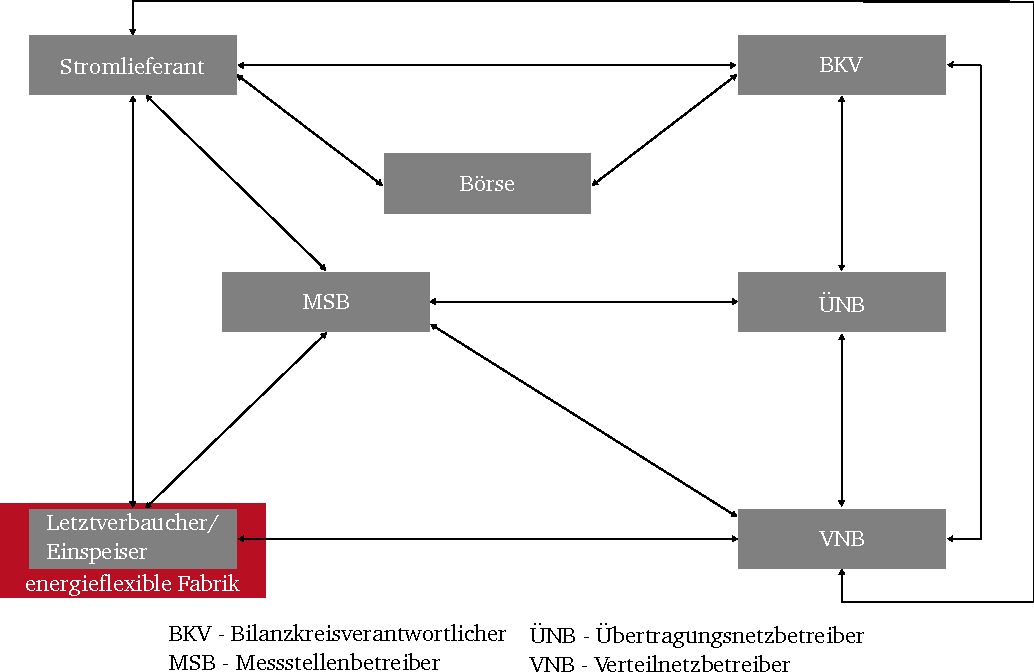
\includegraphics[width=400pt]{figures/03_Grundlagen/Vertragsbeziehungen zwischen den Akteuren am Strommarkt.pdf}
	\caption{Vertragsbeziehungen zwischen den Akteuren am Strommarkt, nach \cite{VDI5207Blatt2020}}
	\label{fig_03Vertragsbeziehungen zwischen den Akteuren am Strommarkt}
\end{figure}

Übertragungsnetzbetreiber (ÜNB) sind für den Betrieb und die Instandhaltung der Höchst- und Hochspannungsnetze verantwortlich. Diese Netze transportieren Strom über große Entfernungen und sorgen für die Einspeisung in die Verteilnetze sowie die Aufnahme von Energie aus diesen Netzen. In Deutschland gibt es vier ÜNBs: Amprion, TransnetBW, TenneT und 50Hertz. Gemäß § 12 des Energiewirtschaftsgesetzes (EnWG) sind diese Betreiber verpflichtet, die Versorgungssicherheit zu gewährleisten. Dazu erbringen sie wichtige Systemdienstleistungen wie Frequenzhaltung, Spannungshaltung, Betriebsführung und den Wiederaufbau der Versorgung nach Störungen. Die ÜNBs spielen auch eine zentrale Rolle bei der Integration erneuerbarer Energien in das Stromnetz, da sie die schwankende Einspeisung von Wind- und Solarenergie managen müssen \cite{VDI5207Blatt2020, hammonsIntegratingRenewableEnergy2008}.\\

Verteilnetzbetreiber (VNB) sind für den Betrieb und die Verwaltung der Verteilnetze verantwortlich, welche die Mittelspannungsebene (und teilweise auch die Hochspannungsebene in großen städtischen Gebieten) sowie alle darunterliegenden Spannungsebenen und Umspannstationen umfassen. Ihre gesetzliche Verpflichtung besteht darin, ein sicheres, zuverlässiges und leistungsfähiges Energieversorgungsnetz diskriminierungsfrei zu betreiben, zu warten und bei Bedarf zu optimieren, zu verstärken und auszubauen, sofern dies wirtschaftlich vertretbar ist. In Deutschland gibt es etwa 900 VNBs, die eine zentrale Rolle in der Stromverteilung spielen. Ein wichtiger Aspekt der VNBs ist ihre Beteiligung an DR-Programmen. VNBs stellen zudem Messdienste bereit, die genaue Verbrauchsdaten erfassen und an andere Marktteilnehmer wie ÜNBs und Stromlieferanten weiterleiten. Diese Daten sind essentiell für die Abrechnung und die Planung des Energiebedarfs \cite{VDI5207Blatt2020, stanelyteOverviewDemandResponseServices2022}.\\

Messstellenbetreiber (MSB) in Deutschland spielen eine zentrale Rolle im Energiemarkt, indem sie die Installation und den Betrieb von modernen Messeinrichtungen und intelligenten Messsystemen (Smart Meter) sicherstellen. Gemäß der VDI 5207 Blatt 1 \cite{VDI5207Blatt2020} kann jeder Endverbraucher seinen MSB frei wählen. Die MSBs sind für die Bereitstellung und den Betrieb dieser Messsysteme verantwortlich, die genaue Verbrauchsdaten erfassen und diese über das Smart Meter Gateway an berechtigte Marktteilnehmer weiterleiten. Moderne Messeinrichtungen und intelligente Messsysteme tragen erheblich zur Transparenz und Effizienz im Energiemarkt bei. Durch die präzise Erfassung von Echtzeitdaten ermöglichen sie eine bessere Planung und Optimierung des Energieverbrauchs, was sowohl ökonomische als auch ökologische Vorteile bietet \cite{VDI5207Blatt2020, rindSmartEnergyMeters2023}.\\

Stromlieferanten spielen eine zentrale Rolle im Strommarkt, indem sie elektrische Energie an Endverbraucher verkaufen. Sie beziehen den Strom entweder direkt von Erzeugern oder über Handelsplattformen wie die Börse und verteilen ihn an Haushalte, Unternehmen und industrielle Abnehmer. Die Preisgestaltung erfolgt in der Regel durch die Kombination von variablen Kosten pro verbrauchter Kilowattstunde und festen Grundgebühren, die unabhängig vom individuellen Verbrauch anfallen und für die Wartung des Stromnetzes sowie der Zähler zuständig sind \cite{VDI5207Blatt2020}.\\

Bilanzkreisverantwortliche (BKV) nehmen im Strommarkt eine zentrale Position ein, indem sie das Gleichgewicht zwischen Erzeugung und Verbrauch bzw. der Einspeisung und Entnahme von Strom innerhalb eines Bilanzkreises sicherstellen. Sie fungieren als wichtige Schnittstellen zwischen Verbrauchern und ÜNBs. Die Hauptaufgaben der BKVs umfassen die Erstellung von Prognosen für den Energieverbrauch und die Energieerzeugung sowie die Entwicklung von Handelsstrategien, um dieses Gleichgewicht zu gewährleisten. BKVs überwachen kontinuierlich den Zustand ihres Bilanzkreises und greifen bei Abweichungen zwischen prognostizierten und tatsächlichen Werten ein. Dazu gehören Maßnahmen wie der Handel von Ausgleichsenergie am Regelenergiemarkt, um kurzfristige Ungleichgewichte auszugleichen und die Netzstabilität zu gewährleisten \cite{VDI5207Blatt2020, wawerElektrizitaetswirtschaftPraxisorientierteEinfuehrung2022}.\\ 

Letztverbraucher, zu denen Unternehmen, energieflexible Fabriken und Haushalte zählen, wählen ihren Stromlieferanten basierend auf Kriterien wie Strommix, Preisgestaltung und vertraglichen Bedingungen. Diese Verbraucher zahlen dem gewählten Lieferanten den vereinbarten Strompreis. In einigen Fällen handeln Unternehmen direkt an der Börse oder beauftragen Dienstleister wie Direktvermarkter oder Aggregatoren, um den benötigten Strom zu beschaffen. Dadurch treten sie selbst als Lieferanten auf \cite{VDI5207Blatt2020}. Die Hauptaufgaben der Stromerzeuger und Einspeiser bestehen darin, elektrische Energie zu erzeugen und diese in die Übertragungs- oder Verteilnetze einzuspeisen, abhängig von ihrer Leistungskapazität. Anschließend verkaufen die Erzeuger den produzierten Strom an Handelsplätzen wie der Börse \cite{bardtWettbewerblicherStrommarktFuer2014}.\\

Die dargestellten Vertragsbeziehungen verdeutlichen die komplexe Interaktion zwischen den verschiedenen Akteuren des Strommarktes und unterstreichen die Notwendigkeit einer koordinierten Zusammenarbeit zur Sicherstellung einer stabilen und effizienten Stromversorgung.\\

\subsection{Bedeutung der Marktsegmente}

Abbildung \refeq{fig_03Deutscher Strommarkt} zeigt die verschiedenen Märkte, die für den Handel mit Strom und Flexibilität in Betracht kommen. Diese Märkte haben jeweils spezifische Zugangsbedingungen, einschließlich technischer Anforderungen und Handelslizenzen, die oft mit hinterlegten Bankbürgschaften verknüpft sind. Sollte ein Unternehmen diese Voraussetzungen nicht erfüllen, besteht die Möglichkeit der Teilnahme über einen Stromlieferanten oder Aggregator.

Nach der Betrachtung der einzelnen Akteure und ihrer Rollen im Strommarkt ist es nun entscheidend, die verschiedenen Marktsegmente zu erläutern, die die Grundlage für den Handel und die Preisfindung bilden. Im nächsten Abschnitt wird zunächst die Funktion und Bedeutung der Börse im Strommarkt beschrieben, bevor auf die unterschiedlichen Marktsegmente wie Spotmarkt, Terminmarkt und Regelenergiemarkt eingegangen wird.\\

\begin{figure}[h]
	\centering
	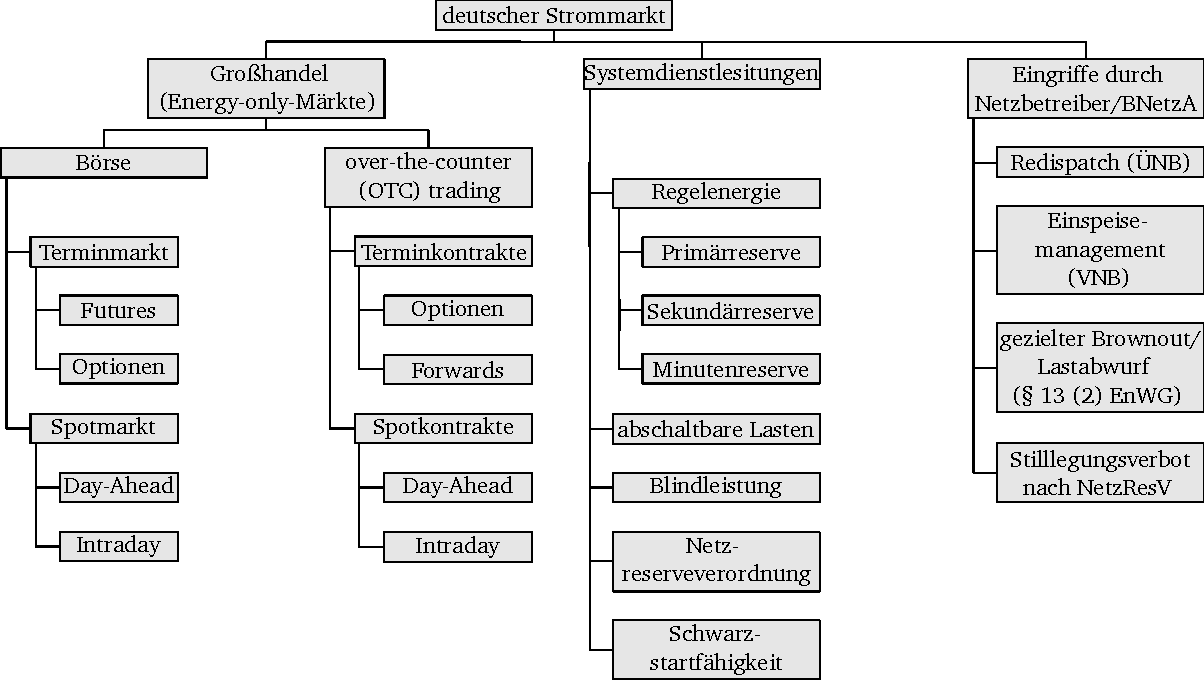
\includegraphics[width=400pt]{figures/03_Grundlagen/Deutscher Strommarkt.pdf}
	\caption{Deutscher Strommarkt, nach \cite{VDI5207Blatt2020}}
	\label{fig_03Deutscher Strommarkt}
\end{figure}
(Linien müssen überarbeitet werden, teilweise nicht genau aufeinander und dicker als die anderen)\\

Der Begriff Energy-only-Märkte bezeichnet alle Energiemärkte, auf denen tatsächliche Stromlieferungen (in Megawattstunden, MWh) kurz vor ihrer Lieferung gehandelt werden. Diese Märkte operieren auf Basis von Angebot und Nachfrage. Preissignale in diesen Märkten lenken sowohl Investitionen als auch den kurzfristig optimalen Einsatz von Ressourcen seitens Erzeugern und Verbrauchern, was aus volkswirtschaftlicher Sicht von Bedeutung ist. Zudem bieten die unterschiedlichen Marktsegmente Möglichkeiten zur Risikominderung durch Hedging, bei dem Finanzkontrakte zur Absicherung bestehender Risiken eingesetzt werden, sowie zur Arbitrage, wo Preisunterschiede zur Gewinnsteigerung genutzt werden können (betriebswirtschaftliche Perspektive). Der Handel findet sowohl an Börsen als auch bilateral über sogenannte Over-the-Counter-Geschäfte (OTC) statt \cite{VDI5207Blatt2020}.\\

Der Handel mit Strom erfolgt an spezialisierten Börsen und ist damit vergleichbar mit dem Aktienhandel. Ein prominentes Beispiel ist die European Energy Exchange (EEX), an der unter anderem auch der Strom für Deutschland gehandelt wird. Es gibt jedoch weitere Börsen, an denen Strom gehandelt wird, wie etwa die Nord Pool oder die Power Exchange Central Europe (PXE).\\

Ein wesentlicher Vorteil des Börsenhandels gegenüber dem OTC-Markt liegt in der hohen Liquidität. Börsen bieten eine standardisierte und transparente Handelsumgebung, die das Risiko für die Marktteilnehmer reduziert und eine verlässliche Preisbildung ermöglicht.\\

An den Strombörsen werden sowohl Spot- als auch Termin- bzw. Future-Kontrakte gehandelt:
Einheiten müssen hier noch als Formel formuliert werden
\begin{itemize}[label={--}]
	
\item \textbf{Spotmarkt:}\\ Der Spotmarkt umfasst Produkte im Stunden- und Viertelstundenraster. Dazu zählen der Day-Ahead-Markt, bei dem Strom für den folgenden Tag gehandelt wird, und der Intraday-Markt, der den kontinuierlichen Kauf und Verkauf von Strom für die Lieferung am selben Tag ermöglicht.\\

Im Day-Ahead-Handel, der an der EEX Spot oder im OTC-Handel stattfindet, können an jedem Tag des Jahres bis 12:00 Uhr mittags Gebote für den kommenden Tag abgegeben werden. Es werden verschiedene Produkte gehandelt, einschließlich voller Stunden und standardisierter Blockgebote, mit einer Mindesthandelseinheit von 0,1 MW und einer maximalen Blockgebotsgröße von 400 MW. Die Auktionsergebnisse, einschließlich des Markträumungspreises, werden um 12:40 Uhr veröffentlicht. Der Markträumungspreis wird durch den Schnittpunkt von Angebots- und Nachfragegeboten bestimmt, was diese Auktion zu einer Einheitspreisauktion macht.\\

Intraday-Märkte ermöglichen den kurzfristigen Stromhandel bis kurz vor der physikalischen Lieferung in viertelstündigen Intervallen. Es gibt eine Eröffnungsauktion sowie einen kontinuierlichen Handel. Die Preisspanne reicht von –9999 EUR/MWh bis +9999 EUR/MWh. Angesichts der zunehmenden Einspeisung erneuerbarer Energien sind diese Märkte besonders wichtig, um auch untertägig auf Preisschwankungen, beispielsweise durch korrigierte Wetterprognosen, reagieren zu können.\\

Diese standardisierten Produkte optimieren die Beschaffung und den Verkauf von Strom und bieten technisch-wirtschaftlich-rechtliche Sicherheiten. Sie ermöglichen es den Marktteilnehmern, Marktpreisrisiken je nach spezifischem Bedarf auszugleichen.\\

\item \textbf{Termin- bzw. Future-Kontrakte:}\\ Termin- bzw. Future-Kontrakte ermöglichen die langfristige Absicherung von Energielieferungen durch den Handel in Wochen-, Monats-, Quartals- und Jahresblöcken. Diese Kontrakte bieten den Marktteilnehmern die Möglichkeit, sich gegen zukünftige Preisschwankungen abzusichern und eine stabile Planungsgrundlage zu schaffen. Darüber hinaus erlauben sie eine Optimierung des Portfolios und die finanzielle Absicherung zukünftiger Liefergeschäfte. Der Handel kann sowohl an der Börse als auch über OTC-Geschäfte (Over-the-Counter) erfolgen. An der Börse ist der Handel bis zu sechs Jahre im Voraus möglich. Mit Futures kann man sich gegen Preisspitzen und Preistiefs absichern. Durch die Optionen können Wochen-, Monats-, Quartals- und Jahres-Futures im Peakload (8:00 - 20:00 Uhr) oder Baseload (24-Stunden-Block) gehandelt werden. Diese Kontrakte sind besonders wichtig als Mittel zur Risikoabsicherung für die fluktuierende Erzeugung erneuerbarer Energien oder für Marktpreisspitzen, die durch den wachsenden Anteil erneuerbarer Energien bedingt sind.
\end{itemize}

Der physische Stromfluss erfolgt unabhängig vom Handel über die Netzbetreiber, die je nach Spannungsebene als ÜNBs oder VNBs fungieren. Die bilanziellen Transaktionen werden durch den BKV bis zum Letztverbraucher abgewickelt.\\

Der Over-the-Counter (OTC)-Handel bezeichnet den bilateralen Handel von Strom, der neben dem Börsenhandel weiterhin eine gängige Methode im Spot-Geschäft darstellt. Im OTC-Handel werden Lieferverträge direkt mit den Abnehmern abgeschlossen, wodurch die Produkte individuell anpassbar sind, beispielsweise auf viertelstündlicher Basis. Die Verkaufserlöse fließen hierbei direkt vom Abnehmer zum Stromerzeuger. Der physische Stromfluss erfolgt auch im OTC-Handel über die Netzbetreiber, während die bilanzielle Abwicklung durch den Bilanzkreisverantwortlichen (BKV) bis zum Letztverbraucher erfolgt.\\

Systemdienstleistungen sind essenzielle Maßnahmen, die dazu dienen, die Stabilität und Sicherheit des Stromnetzes zu gewährleisten. Diese Maßnahmen sorgen dafür, dass die Netzfrequenz, die Spannung und die Leistungsbelastungen innerhalb festgelegter Grenzen bleiben oder nach Störungen wiederhergestellt werden. Üblicherweise werden diese Maßnahmen von den Netzbetreibern koordiniert und ausgeführt. Bei Störungen im Netz werden marktbezogene Interventionen wie Regelenergie und Engpassmanagement eingesetzt, ebenso wie steuerbare Lasten, die je nach Bedarf zu- oder abgeschaltet werden können. Darüber hinaus stehen Reservekapazitäten zur Verfügung, um die Netzstabilität und die Versorgungssicherheit auch in kritischen Situationen aufrechtzuerhalten.\\

\begin{itemize}[label={--}]

\item \textbf{Regelleistungsmarkt:}\\
Der Regelleistungsmarkt spielt eine entscheidende Rolle beim kurzfristigen Ausgleich von Stromangebot und -nachfrage nach Handelsschluss bis zum Zeitpunkt der physischen Lieferung. Dies dient der Aufrechterhaltung der Netzstabilität und der Sollfrequenz von 50,0 Hz. Teilnahmeberechtigt sind nur präqualifizierte Akteure, die eine vorwettbewerbliche Eignungsprüfung bestanden haben und die technischen Voraussetzungen zur Erbringung der Regelleistung erfüllen.

\begin{itemize}[label={--}]
\item \textbf{Positive Regelenergie} wird benötigt, wenn die Nachfrage das Angebot übersteigt.
\item \textbf{Negative Regelenergie} kommt zum Einsatz, wenn die Nachfrage unter dem Angebot liegt.
\end{itemize}

Die Verantwortung für den Regelleistungsmarkt liegt bei den ÜNB. Es gibt drei Typen von Regelreserve: Primärregelleistung, Sekundärregelleistung und Minutenreserveleistung. Diese unterscheiden sich hinsichtlich ihres Zeithorizonts und ihrer Anforderungen an die Anbieter.\\

\item \textbf{Verordnung zu ab- und zuschaltbaren Lasten:}\\
Die Verordnung zu abschaltbaren Lasten regelt die Steuerung von Stromverbrauchern durch den ÜNB bei Netzengpässen. Dabei können bestimmte Lasten gezielt reduziert werden. Man unterscheidet hierbei zwischen schnell und sofort abschaltbaren Lasten. Anbieter solcher Lasten müssen spezifische technische Anforderungen erfüllen und einen Rahmenvertrag mit dem ÜNB abschließen. Die Ausschreibungen für abschaltbare Lasten sind vor allem auf industrielle Verbraucher zugeschnitten, im Gegensatz zu den Anforderungen der Regelenergie. Die Verordnung zu zuschaltbaren Lasten funktioniert ähnlich wie die Bereitstellung negativer Regelenergie. Flexible Industrieprozesse können diese Art von Last anbieten. Diese Flexibilität steht dem ÜNB zur Verfügung und kann im Falle eines Netzengpasses genutzt werden, um die Netzstabilität zu sichern.\\
\end{itemize}

Die Kapazitätsreserve ist ein zentrales Instrument, das durch das Gesetz zur Weiterentwicklung des Strommarktes eingeführt wurde, um die Systemverantwortung der Übertragungsnetzbetreiber (ÜNB) zu gewährleisten. Diese Reserve dient der Bewältigung von Netzengpässen, der Stabilisierung der Netzspannung und der Wiederherstellung der Stromversorgung nach Störungen. Für die Kapazitätsreserve kommen Anlagen infrage, die zwar momentan nicht in Betrieb sind, aber aufgrund ihrer Systemrelevanz – beispielsweise ihrer Position im Netz – von den ÜNB reaktiviert werden können. Diese Anlagen werden in die Kapazitätsreserve integriert, um bei Bedarf die Stabilität und Zuverlässigkeit des Stromnetzes sicherzustellen.\\

Im Flexibilitätsmarkt nehmen Aggregatoren eine entscheidende Position ein. Sie bündeln die Flexibilität vieler kleiner Unternehmen und bieten diese gebündelt den Netzbetreibern an. Einzelne kleine Akteure sind für Netzbetreiber meist uninteressant, da größere Flexibilitätspakete bevorzugt werden. Unternehmen, die Flexibilität zur Verfügung stellen, werden dafür finanziell entschädigt. Ein Beispiel hierfür ist die Regelenergie, die von Übertragungsnetzbetreibern (ÜNB) genutzt wird, wenn der Bedarf hoch ist, etwa bei speziellen Wetterbedingungen wie Frühnebel. In solchen Situationen können gesteuerte Industrieanlagen eine wichtige Rolle spielen. Aggregatoren übernehmen auch eine Versicherungsfunktion. Sollte ein Unternehmen vorübergehend nicht in der Lage sein, Flexibilität zu bieten, können Aggregatoren die erforderliche Flexibilität durch andere Unternehmen bereitstellen. Dies ist besonders für kleine Unternehmen vorteilhaft, da sie alleine oft nicht genügend Flexibilität anbieten können. Es besteht jedoch ein Bedarf an gesetzlicher Anpassung, da der politische Fokus derzeit noch stark auf Energieerzeugung und weniger auf das Lastmanagement gerichtet ist. Der Flexibilitätsmarkt eröffnet Möglichkeiten für verschiedene Akteure, einschließlich Unternehmen, kleinerer Betriebe und Haushalte, sich aktiv an der Netzstabilisierung zu beteiligen. Ein Beispiel dafür ist die Modellstadt Augsburg, wo auch Haushalte am Flexibilitätsmarkt teilnehmen und somit zur Netzstabilität beitragen können \cite{Projektziel}.\\ (Zitat in Zotero noch ergänzen)

\subsection{Abgaben und Umlagen}
Letztverbraucher tragen neben den Vertriebskosten des Stromlieferanten, die je nach Menge und Zeitpunkt des Stromverbrauchs variieren, auch diverse administrative Preisbestandteile. Dazu zählen die Strom- und Mehrwertsteuer sowie verschiedene Umlagen, wie die des Erneuerbare-Energien-Gesetzes (EEG), des Kraft-Wärme-Kopplungsgesetzes (KWKG) und der Stromnetzentgeltverordnung (StromNEV). Weitere Kostenpunkte sind die Umlage für abschaltbare Lasten, die Konzessionsabgabe und die Netzentgelte. Diese Abgaben und Umlagen werden jährlich von der Bundesnetzagentur festgelegt.\\


In der Abbildung \refeq{ch_09Methodenkritik und Limitation der durchgeführten Untersuchung} wird die Aufteilung des Einzelhandelspreisniveaus für Haushaltskunden im Abnahmeband von 2.500 bis 5.000 kWh pro Jahr zum 1. April 2023 dargestellt. Die größten Kostenanteile entfallen auf die Energiebeschaffung mit 40,6 \% und die Nettonetzentgelte mit 19,9 \%. Weitere bedeutende Posten sind die Umsatzsteuer (16,0 \%), Vertrieb und Marge (11,6 \%) sowie die Stromsteuer (4,5 \%). Kleinere Anteile werden durch die Konzessionsabgabe (3,6 \%), das Entgelt für Messung und Messstellenbetrieb (0,8 \%) sowie verschiedene Umlagen wie die Umlage nach KWKG, nach §19 StromNEV und die Offshore-Netzumlage abgedeckt. Diese Struktur verdeutlicht, wie sich die Kosten für Strom für Endverbraucher zusammensetzen und welche Anteile durch gesetzliche Abgaben und Umlagen beeinflusst werden.
Quelle Bundesnetzagentur muss in Zotero noch ausgebessert werden!
\begin{figure}[h]
	\centering
	\includegraphics[width=400pt]{figures/03_Grundlagen/Aufteilung des Einzelhandelspreisniveaus für Haushaltskunden für das Abnahmeband ab einschließlich 2.500 bis 5.000 kWh pro Jahr zum 1. April 2023.pdf}
	\caption{Aufteilung des Einzelhandelspreisniveaus für Haushaltskunden für das Abnahmeband ab einschließlich 2.500 bis 5.000 kWh pro Jahr zum 1. April 2023 , nach \cite{BundesnetzagenturMonitoringberichte}}
	\label{fig_03Aufteilung des Einzelhandelspreisniveaus für Haushaltskunden für das Abnahmeband ab einschließlich 2.500 bis 5.000 kWh pro Jahr zum 1. April 2023}
\end{figure}
Bild muss noch ausgebssert werden - Kreis ganz rund machen

Stromintensive Unternehmen profitieren von speziellen Regelungen bei der EEG-Umlage: Ab einem bestimmten Verbrauchsniveau zahlen sie nicht mehr den vollen Umlagebetrag. Ähnlich verhält es sich bei der KWKG-Umlage, die ebenfalls von allen Stromverbrauchern landesweit getragen wird, jedoch für besonders stromintensive Betriebe begrenzt ist.

Noch was zum Merit-Order Effekt fehlt und zur EEG-Umlage 
%Es kann auf andere Kapitel, Gleichungen, Tabellen und Abbildungen verwiesen werden über Labels. Hier Beispiele: Kapitel \ref{ch_03Grundlagen1_1}, Gleichung (\ref{equ_03Grundlagen1_1_1_2}),
%Tabelle \ref{tab_03Grundlagen1_1_1},
%Abbildung \ref{fig_03Fourier1}
%
%Es ist Sinnvoll auf die Abbildungen und Tabellen immer mit Hilfe dieser Labels zu verweisen, da die Position dieser im Text von TeX so bestimmt wird, dass sich ein gleichmäßiges Schriftbild ergibt. Hierdurch kommen die Abbildungen und Tabellen nicht immer an der Stelle zum liegen an der sie im Code eingefügt sind.
%
%Die Vergebenen Labels müssen immer eindeutig sein. Die Nummerierung bei den Labels wird von TeX immer automatisch beim kompilieren aktualisiert. Ist ein Label nicht Vorhanden beispielsweise aufgrund eines Schreibfehlers, werden an der entsprechenden Stelle Fragezeichen eingefügt, wie hier \ref{Fantasielabel}. Deshalb kann es Sinnvoll sein Stellen an denen noch etwas zu bearbeiten ist mit Fragezeichen zu kennzeichnen und am Ende das Dokument über die Suchfunktion nach Fragezeichen zu durchsuchen, um nichts zu vergessen und Fehler in den Labels zu entdecken.
%
%Bei den Quellenverweisen wird in ähnlicher Form mit Labels gearbeitet. Die Daten zu den Literaturquellen sind in der bib-Datei im bibliography-Ordner hinterlegt. In dieser Datei sind für die Literatur-Einträge auch Labels hinterlegt, welche hier z.B. \cite{Binder.2017} oder optional mit Angabe der Seitenzahl \cite[S.666]{Binder.2017} oder als Aufzählung \cite{Bianchi.2009, Kerdsup.2014, Sanada.2003, Howard.2015} aufgerufen werden können. Die bib-Datei kann entweder händisch erstellt werden (nicht zu empfehlen) oder z.B. über ein Literaturverwaltungsprogramm wie Citavi. Die Labels(bibtex-keys) können in Citavi verändert werden und werden dann beim nächsten Export der bib-Datei eingetragen.


%\subsection{Grundlagen1\_1}
%\label{ch_03Grundlagen1_1}
%Beispiel für eine Aufzählung:
%
%Bei den vereinfachenden Annahmen handelt es sich um die Folgenden \cite{Binder.2017}:
%\begin{itemize}
%\item Das Eisen wird als näherungsweise unendlich magnetisch leitfähig (ideales Eisen) angenommen $\mu_{\textsf{Fe}} \to \infty$.
%\item Das Luftspaltfeld besitzt nur eine radiale Komponente, da die Luftspaltweite $\delta$ viel kleiner ist als die Polteilung $\tau_{\textsf{P}}$. 
%\item Es wird ein ebenes zweidimensionales Feld vorausgesetzt; Randeffekte an den Enden der Maschine werden vernachlässigt.
%\item Die Spulen und die Nuten, in denen diese liegen, werden als punktförmig angenommen (\textit{Dirac}'sche Durchflutungsimpulse).
%\end{itemize}
%
%Für die Erstellung von Tabellen sei auch auf hilfreiche Seiten wie https://www.tablesgenerator.com verwiesen. 
%
%\begin{table}[h]
%	\begin{center}
%		\caption[Maschinen-Kenndaten der ausgewählten Rotorblechschnittvarianten]{Maschinen-Kenndaten der ausgewählten Rotorblechschnittvarianten für den Betriebspunkt $I_\textsf{S}=1.6\,\textsf{A}$, $\beta =55°$}
%		\begin{tabular}{c|c|c|c|c|}
%		\cline{2-5}
%		                       	    & Variante 1A & Variante 1B & Variante 2A & Variante 2B \\ \hline
%		\multicolumn{1}{|c|}{$M_\textsf{e,mean}$} & $5.39\,\textsf{Nm}$ & $5.37\,\textsf{Nm}$ & $5.32\,\textsf{Nm}$ & $5.28\,\textsf{Nm}$ \\ \hline
%		\multicolumn{1}{|c|}{$\Delta M_\textsf{e,rel}$} & $8.78\,\%$ & $8.97\,\%$ & $4.52\,\%$ & $4.33\,\%$ \\ \hline
%		\multicolumn{1}{|c|}{$\cos\left(\varphi_\textsf{S} \right)$ für $R_\textsf{S}=0$} & $0.716$ & $0.720$ & $0.719$ & $0.717$ \\ \hline
%		\multicolumn{1}{|c|}{$\max\left(M_\textsf{e} \right)$} & $5.67\,\textsf{Nm}$ & $5.64\,\textsf{Nm}$ & $5.44\,\textsf{Nm}$ & $5.42\,\textsf{Nm}$ \\ \hline
%		\multicolumn{1}{|c|}{$\min\left(M_\textsf{e} \right)$} & $5.20\,\textsf{Nm}$ & $5.16\,\textsf{Nm}$ & $5.20\,\textsf{Nm}$ & $5.19\,\textsf{Nm}$ \\ \hline
%		\end{tabular}
%		\label{tab_03Grundlagen1_1_1}
%	\end{center}
%\end{table}
%
%\subsubsection{Grundlagen1\_1\_1}
%\label{ch_03Grundlagen1_1_1}
%In Abbildung \ref{fig_03Grundlagen1_1_1_1} ist ein Beispielbild zu sehen welches mit Inkscape erstellt worden ist. Die Bildunterschrift in eckigen Klammern ist die gekürzte Version für das Abbildungsverzeichnis und in geschweiften Klammern steht die ausführliche Beschreibung. Dies gilt ebenfalls für die Tabelle \ref{tab_03Grundlagen1_1_1}. 
%
%\begin{figure}[h]
%\centering
%\def\svgwidth{400pt}
%\input{figures/03_Grundlagen/Spule_2_poliger_Motor.pdf_tex}
%\caption[Zweipoliger Motor mit einer Ständerspule und homogenem Rotor]{Zweipoliger Motor mit einer Ständerspule und homogenem Rotor: \textbf{a)} Querschnitt und Feldlinien $\vec{B}$ in Folge der Nutdurchflutung $\Theta_\textsf{Q}$; \textbf{b)} Skizze des Flussdichteverlaufs $B(x)$ und Strombelags $A_\textsf{S}(x)$ über dem Luftspaltumfang $x$, nach \cite{Binder.2017}}
%\label{fig_03Grundlagen1_1_1_1}
%\end{figure}
%
%Um die Flussdichte $B_\delta$ im Luftspalt quantitativ mit dem Stromfluss $i_\textsf{C}$ in der Wicklung in Verbindung zu bringen, werden das Gesetz vom magnetischen Hüllenfluss
%%
%\begin{equation}
%\label{equ_03Grundlagen1_1_1_1}
%\oint\limits_A \vec{B} \,\text{d}\vec{A} = 0,
%\end{equation}
%%
%der Durchflutungssatz von \textit{Ampère}
%%
%\begin{equation}
%\label{equ_03Grundlagen1_1_1_2}
%\oint\limits_C \vec{H} \,\text{d}\vec{s} = \Theta
%\end{equation}
%%
%und das Materialgesetz
%%
%\begin{equation}
%\label{equ_03Grundlagen1_1_1_3}
%\vec{B} = \mu(H) \cdot \vec{H}
%\end{equation}
%%
%benötigt \cite{Binder.2017}.
%
%\subsubsection{\textit{Fourier}-Reihenentwicklung der Felderregerkurve}
%\label{ch_03Fourier}
%Die \textit{Fourier}-Reihe einer $2\pi$-periodischen Funktion $V(\gamma)$ lässt sich in der folgenden Form darstellen \cite{Binder.2017}:
%
%\begin{equation}
%\label{equ_03Fourier1}
%V(\gamma) = V_\textsf{mean} + \sum\limits_{\nu=1,2,3...}^\infty \left \lbrack \hat{V}_{\nu\textsf{,a}} \cdot \cos(\nu \gamma) + \hat{V}_{\nu\textsf{,b}} \cdot \sin(\nu \gamma) \right \rbrack
%\end{equation}
%
%Die Amplituden der Harmonischen $\hat{V}_{\nu\textsf{, a}}$ und $\hat{V}_{\nu\textsf{, b}}$ mit den Ordnungszahlen $\nu$ berechnen sich aus den Integralen (\ref{equ_03Fourier2}) und (\ref{equ_03Fourier3}) \cite{Binder.2017}.
%%
%\begin{equation}
%\hat{V}_{\nu\textsf{, a}} = \frac{1}{\pi} \int\limits_{0}^{2\pi} V(\gamma) \cdot \cos(\nu\gamma) \,\text{d}\gamma
%\label{equ_03Fourier2}
%\end{equation}
%%
%%
%\begin{equation}
%\hat{V}_{\nu\textsf{, b}} = \frac{1}{\pi} \int\limits_{0}^{2\pi} V(\gamma) \cdot \sin(\nu\gamma) \,\text{d}\gamma
%\label{equ_03Fourier3}
%\end{equation}
%%
%Die Konstante $V_\textsf{mean}$ stellt den Mittelwert der periodischen Funktion $V(\gamma)$ dar und ergibt sich aus dem Integral (\ref{equ_03Fourier4}) \cite{Binder.2017}.
%%
%\begin{equation}
%V_\textsf{mean} = \frac{1}{2\pi} \int\limits_{0}^{2\pi} V(\gamma) \,\text{d}\gamma
%\label{equ_03Fourier4}
%\end{equation}
%%
%
%\begin{figure}[h]
%\centering
%\def\svgwidth{490pt}
%\input{figures/03_Grundlagen/Fourier_1_Spule.pdf_tex}
%\caption[Felderregerkurve $V_\textsf{C}(\gamma)$ einer Spule eines Strangs einer Einschichtwicklung]{Felderregerkurve $V_\textsf{C}(\gamma)$ einer Spule eines Strangs einer Einschichtwicklung, nach \cite{Binder.2017}}
%\label{fig_03Fourier1}
%\end{figure}
%
%\subsubsection{Luftspaltleitwert}
%\label{ch_03Nutoeffnung}
%
%Die Grafik \ref{fig_03Nutoeffnung1} wurde mit Python erstellt und als svg-Datei (Vektorgrafik) abgespeichert. Anschließend wurden in Inkscape noch kleine Korrekturen der Achsen Beschriftungen vorgenommen.
%\begin{figure}[h]
%\centering
%\def\svgwidth{340pt}
%\input{figures/03_Grundlagen/dimensionslose_Leitwertfunktion.pdf_tex}
%\caption[Berechnete dimensionslose Leitwertfunktion $\tilde{\lambda}(\gamma)$ für einen vierpoligen Stator]{Berechnete dimensionslose Leitwertfunktion $\tilde{\lambda}(\gamma)$ für einen vierpoligen Stator mit $Q=36$ Nuten}
%\label{fig_03Nutoeffnung1}
%\end{figure}